
\documentclass[twocolumn]{article}
% \documentclass[reprint, twocolumn]{revtex4-2} %formato
\usepackage{graphicx} % graficos
\usepackage{amsmath} %matrices
\usepackage{float}    
\usepackage{hyperref}


\graphicspath{{Imagenes/}} %graficos

\usepackage[spanish]{babel} %idioma


\spanishdecimal{.}
\setlength{\parskip}{1em} 

\begin{document}

% \preprint{APS/123-QED}
\title{Espectroscopía}
\author{Jesús Armando Cañas }
% \affiliation{Universidad de Antiquia}
\author{Miguel Angel Perdomo}
% \affiliation{Universidad de Antiquia}
\date{\today}

\maketitle
\section{Marco teórico}

\subsection{Ley de Planck}
Un cuerpo negro, es una sustancia capaz de absorber toda la radiación térmica que
incide sobre ella\cite{zemansky}. Aunque, se puede suponer que no emite luz porque absorbe todo, si emite luz denominada cuerpo negro, esta luz emitida se puede calcular con la siguiente ecuación denominada ley de Planck.

\begin{equation}
    E(v,T)= \frac{2\pi h c^2}{\lambda^5}\frac{1}{e^{\frac{hc}{K \lambda T}}-1}
    \label{eq: Ley de planck}
\end{equation}
\subsection{Excitación}
Cuando un electrón sufre un proceso de transición de un estado de energia a otro se dice que sufre un proceso de desexitación o excitación. Si el electrón se eleva por cualquier medio a un estado de energía
mayor, se dice que el átomo o el electrón están excitados. El átomo pierde la energía adquirida temporalmente, cuando el electrón regresa a un nivel más bajo y emite
energía radiante, un fotón cuya frecuencia es directamente proporcional a su energía.\cite{Hewitt2007Conceptual}

\[
E = hf
\]
\subsubsection{Espectros de emisión}
Todo elemento tiene una distribución característica de niveles electrónicos de
energía y, en consecuencia, emite luz con su propia distribución de frecuencias, es
decir, su espectro de emisión, cuando se excita.\cite{Hewitt2007Conceptual}

\subsubsection{Espectros de absorción}
Cuando se hace incidir luz atravez de alguna sustancia y luego se analiza la luz transmitida, se obsesrva lo que se denomina el espectro de absorción.
Los átomos absorben la luz, y también la emiten. Un átomo absorbe más la
luz que tenga las frecuencias a las que esté sintonizado: algunas de las mismas fre
cuencias de las que emite. Esta
luz absorbida se vuelve a irradiar, pero en todas direcciones, en vez de sólo en la
dirección del rayo incidente. Cuando la luz que queda en el haz se reparte en
el espectro, las frecuencias que fueron absorbidas aparecen como líneas oscuras
contra el espectro, por lo demás continuo.\cite{Hewitt2007Conceptual}

\subsection{Calibración del espectrometro}
El estándar principal para la escala de radiancia espectral mantenida en la Instalación de Calibraciones Espectrorradiométricas Automatizadas (FASCAL) del Instituto Nacional de Estándares y Tecnología es un cuerpo negro que opera a la temperatura de congelación del oro.\cite{Early1996Irradiance}Que es dado por la ecuacion \ref{eq: Ley de planck}.

La manera en la que se calibran los espectrometros digitales para aquellos dectetores que presentan respuestas con comportamientos lineales, viene dada por la ecuacón:
\[
    S(\lambda)= E(\lambda)\cdot R(\lambda) + D(\lambda)
\]

$S(\lambda)$ es la señal medida por el detector del espectrorradiómetro, $E(\lambda)$ es la irradiancia espectral de la lámpara, $R(\lambda)$ es la respuesta a la irradiancia espectral del espectrorradiómetro y $D(\lambda)$ señal medidad en oscuridad. \cite{Rammeloo2023Spectroradiometer}
Si se linealiza y normaliza la ecuación anterior se obtiene la siguiente ecuación:
\begin{equation}
    E_{\lambda}= B_{\lambda}(\frac{S_{\lambda}-D_{\lambda}}{R_{\lambda}-D_{\lambda}})
    \label{eq: ecuación de transferencia radiométrica relativa}
\end{equation}


\subsection{Bondad de ajuste y test de hipótesis}

Inicialmente, una hipótesis es aquella suposición que se plantea respecto a alguna población o problema con el fin de verificar su veracidad o falsedad. Adicionalmente, una hipótesis nula $H_0$ es aquella hipótesis que inicialmente se asume como cierta con la finalidad de verificarla o falsarla, y la hipótesis alternativa $H_a$ será una suposición que sea contraria a la hipótesis nula. Cabe aclarar que tanto la hipótesis nula como la alternativa deben ser mutuamente excluyentes (contrarias entre sí). Se le llama test de hipótesis a aquel proceso mediante el cual se busca aceptar o rechazar la hipótesis nula. Sin embargo, cabe añadir que este es un proceso probabilístico y no absoluto; por lo cual, que la hipótesis nula sea verdadera o falsa no es un hecho inequívoco. Para poder verificar o falsar la hipótesis nula, existen múltiples herramientas, como la llamada \textit{prueba de bondad de ajuste}, con la cual podemos determinar si ciertos datos experimentales se ajustan a una distribución determinada \cite{marques1991probabilidad}.

\subsection{Distribución chi-cuadrado}
\label{seccion chi}
Si se considera que ciertos datos siguen una distribución determinada, se puede establecer que un evento $E_k$ ocurre con una frecuencia observada $O_k$. Según la distribución teórica, los datos siguen una frecuencia esperada $e_k$; luego, $\chi^2$ se define como \cite{marques1991probabilidad}:

\begin{equation}
\chi^2 = \sum_{k=1}^{n} \frac{(O_k - e_k)^2}{e_k} 
\label{chi}
\end{equation}

Finalmente, tras obtener el estadístico de la distribución chi-cuadrado, es necesario considerar cómo se va a concluir y bajo qué condiciones se determinará que la hipótesis nula se cumple. Así, se define el nivel de significancia ($\alpha$) como la probabilidad de rechazar la hipótesis nula aunque esta sea cierta. Usualmente, en física experimental se emplea un nivel de significancia igual al 5\% \cite{marques1991probabilidad}.


\section{Resultados}
\subsection{Datos de la ley de planck obtenidos experimentalmente}
\begin{figure}[ht]
    \centering
    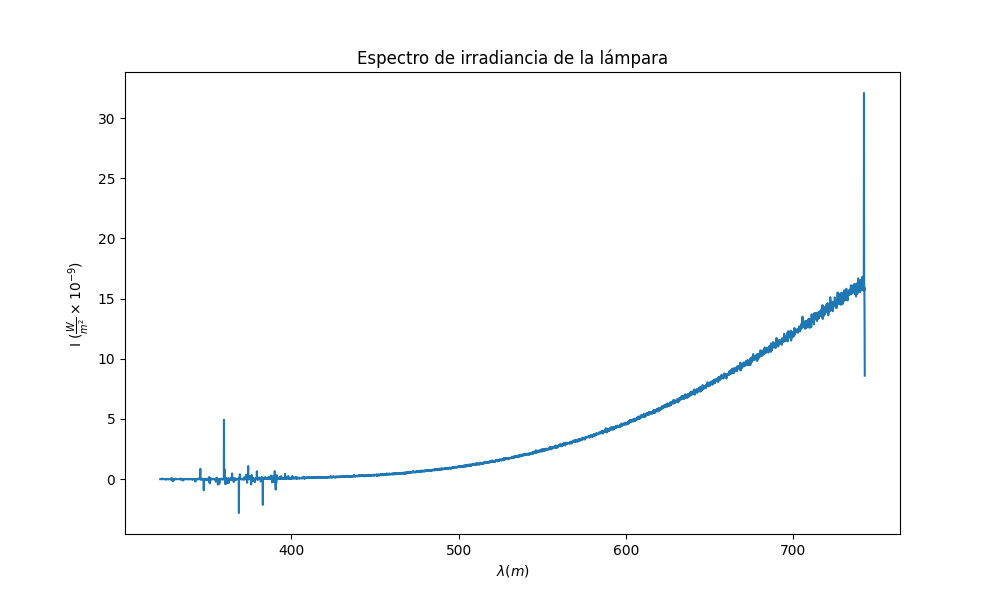
\includegraphics[width =1\linewidth]{Espectro_de_irradiancia_de_la_lampara.png}
    \label{fig: ley de planck}
\end{figure}
Al aplicar la ecuación de la sección se obtuvó el comportamiento de la intensidad ($I$) en función de la longitud de onda ($\lambda$) mostrado en la gráfica \ref{fig: ley de planck}

\subsection{Ajuste de la ley de planck}
\begin{figure}[ht]
    \centering
    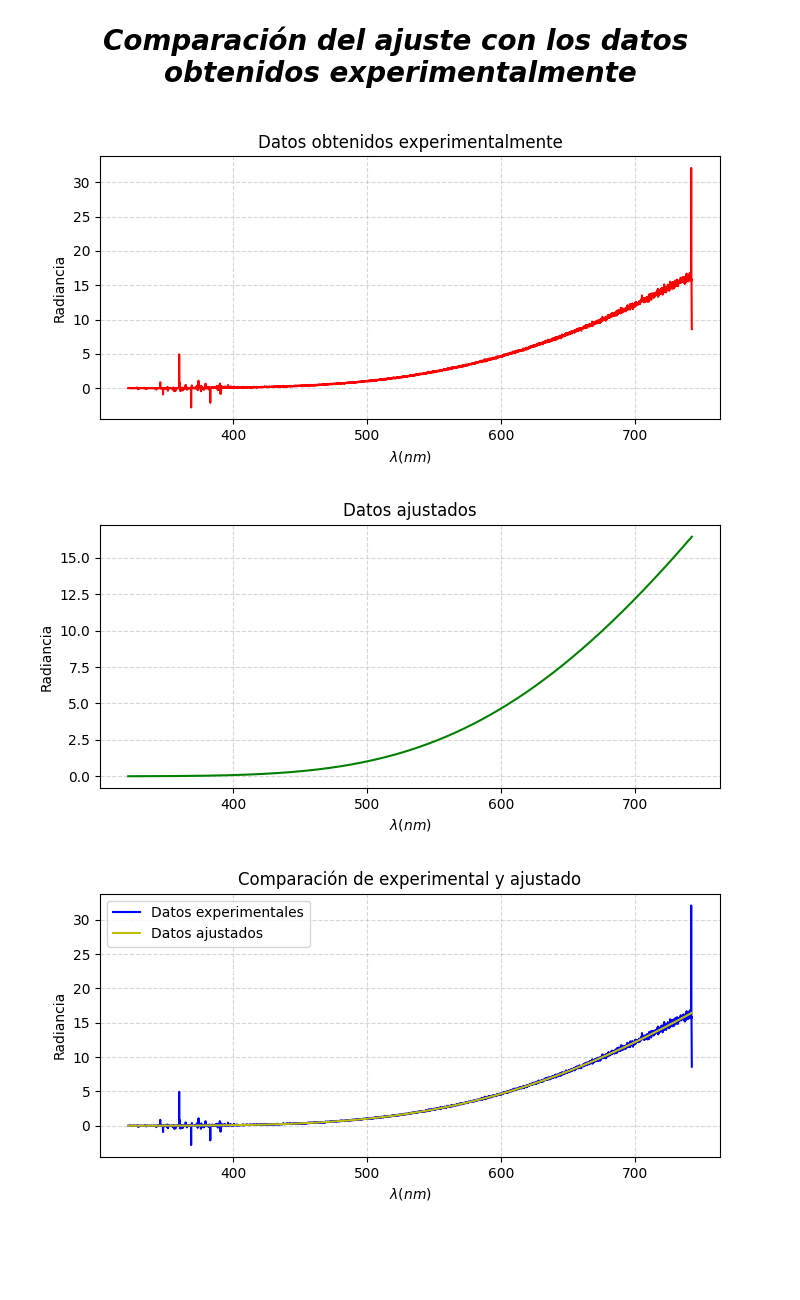
\includegraphics[width =1\linewidth]{Comparación_con_el_ajuste.png}
    \label{fig: Ajuste de la ley de planck}
\end{figure}

En la figura \ref{fig: Ajuste de la ley de planck} se muestra el resultado del ajuste de
la ley de planck al aplicar un ajuste exponencial a la ecuación \ref{eq: Ley de planck}. Visualmente el ajuste es perfecto para modelar la ley de planck. Esto se pudo comprobar mediante el test de Chi cuadrado:

\subsection{Aplicación del test de $\chi^2$}

\begin{figure}[ht]
     \centering
     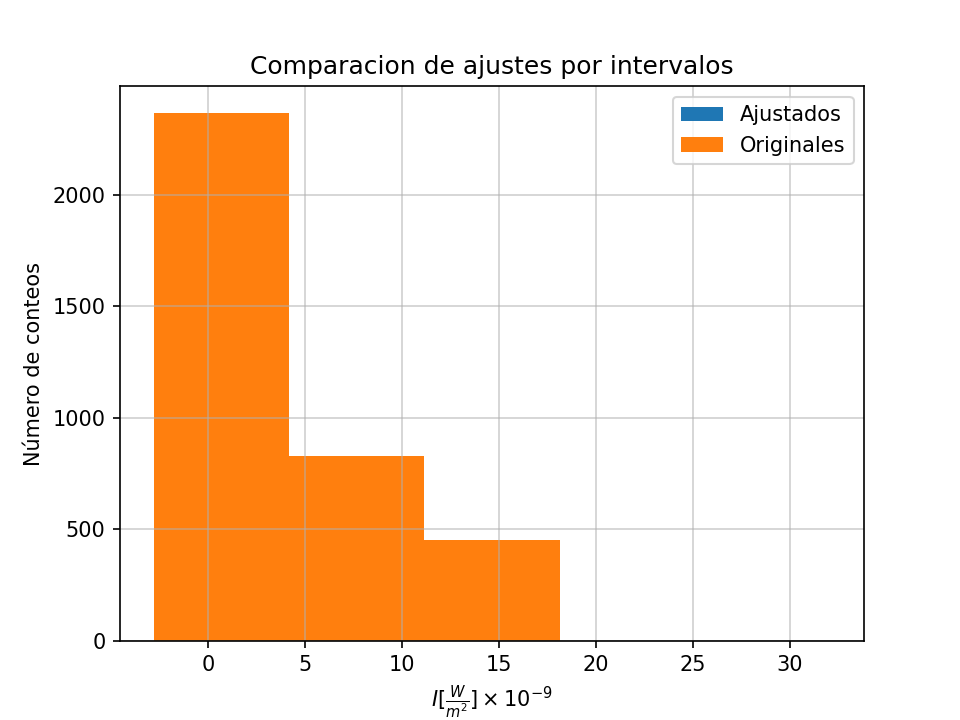
\includegraphics[width =1 \linewidth]{Comparación_con_barras.png}
     \label{fig: aplicación del test}
     \caption{Representación gráfica del número de conteos de intensidades para el test de $\chi^2$}
\end{figure}
En la figura \ref{fig: aplicación del test} se muestra el gráfico de conteos para 5 intervalos de intensidades, para los datos ajustados y los datos obtenidos experimentalmente. Al aplicar el test de $\chi^2$, visto en la sección \ref{seccion chi}, a los conteos obtenidos. Se obtuvo un valor de :
\[
\chi^{2} = 0.04
\]


\bibliographystyle{plain}
\bibliography{EspectroscopiaNotes}

\end{document}